\section{Literature review}\label{sec:state_of_art}

Certainly, in general \gls{ML} classification tasks \footnote{In this
  work, image segmentation is considered as a particular case of classification
in which target classes are assigned pixel-wise.} where multiple
annotators are involved, \gls{MV} is by far the simplest
possible approach to implement. This concept was born multiple times
and divergently in multiple fields, but it was described as relevant
for \gls{ML} and pattern recognition labeling for classification in
\cite{LamAndSuen1997}, in which the approach is exposed as simple,
yet powerful. The authors describe the \gls{MV} as a method that can
be used to improve the accuracy of classification tasks by combining
the labels of multiple annotators. The method is based on the
assumption that the majority vote of the annotators is more likely to
be correct than the vote of a single annotator. The authors also
describe the method as a straightforward way to improve the accuracy
of classification tasks without the need for complex algorithms or
additional data. The authors also prove this method to deliver very
similar results to more complicated approaches (Bayesian, logistic
regression, fuzzy integral, and neural network) in the
particular task of \gls{OCR}. Despite its simplicity, modern
solutions for delivering accurate medical image segmentation models
still rely on Majority Voting at some stage, like \cite{Elnakib2020},
which uses a majority voting strategy for delivering a final output
based on the labels of multiple models (VGG16-Segnet, Resnet-18 and
Alexnet) in \gls{CT} images for Liver Tumor Segmentation, or
\cite{Lopez2023}, which uses \gls{MV} for combining noisy annotations
as an additional annotator to be included in the deep learning solution.
Majority voting as a technique for setting a pseudo ground truth label
is a powerful approach for its simplicity in many use cases in which
the target to be labeled is not tied to an expertise related task,
otherwise, the assumption of equal expertise among the labelers can
be a source of bias in the final label, which is not desirable in the
case of highly technical annotations like medical images.
In subsection \ref{subsec:expertise_levels_lit_review}, we will be
reviewing literature which no longer assumes the naive approach of
equal expertise among labelers and face the challenge of learning
from inconsistent labels.

\subsection{Facing annotation variability in medical
images}\label{subsec:expertise_levels_lit_review}

Learning from crowds approaches in general face the challenge of
not having a ground truth label and hence, an intrinsic difficulty in
measuring the real reliability of the labelers annotations. Some
approaches assume beforehand a certain level of expertise for each
labeler based on experience as an input, like in
\cite{TianEtZhu2015}, which introduce the concept of max margin
majority voting, using the reliability vector as weights for the
weights for the binary and multiclass classifier. The crowdsourcing
margin is the minimal difference between the aggregated score of the
potential true label and the scores for other alternative labels.
Accordingly, the annotators' reliability is estimated as generating
the largest margin between the potential true labels and other
alternatives. The problem introduced in this approach is assuming an
stationary reliability per expert across the whole input space, which
is imprecise since annotators performance may change between
different tasks or even between different regions of the same image.

% REVIEW
\subsubsection{STAPLE Mechanism}

The \gls{STAPLE} algorithm, introduced in \cite{WarfieldEtAl2004}
is a probabilistic framework that estimates a hidden true
segmentation from multiple segmentations provided by
different raters. It also estimates the reliability of each rater by
computing their sensitivity and specificity.

The \gls{STAPLE} algorithm's goal is to maximize the log likelihood function:

\begin{equation}\label{eq:staple_likelilhood}
  (\mathbf{\hat{p}}, \mathbf{\hat{q}}) = \arg\max_{\mathbf{p}, \mathbf{q}} \ln
  f(\mathbf{D},
  \mathbf{T} \mid \mathbf{p}, \mathbf{q}).
\end{equation}

Where $\mathbf{D}$ is the set of segmentations provided by the raters,
$\mathbf{T}$ is the hidden true segmentation, $p$ is the sensitivity
and $q$ is the specificity of the raters.

This is achieved by using the Expectation-Maximization algorithm to
maximize the log likelihood function in equation, which is done iteratively
with step computations:

\begin{equation}
  \begin{split}
    (p_j^{(k)}, q_j^{(k)}) = \arg\max_{p_j, q_j} \sum_{i:D_{ij}=1}
    W_i^{(k-1)} \ln p_j \\
    &+ \sum_{i:D_{ij}=1} \left(1 - W_i^{(k-1)}\right) \ln (1 - q_j) \\
    &+ \sum_{i:D_{ij}=0} W_i^{(k-1)} \ln (1 - p_j) \\
    &+ \sum_{i:D_{ij}=0} \left(1 - W_i^{(k-1)}\right) \ln q_j.
  \end{split}
\end{equation}

The capacity of STAPLE to accurately estimate the true segmentation,
even in the presence of a majority of raters generating correlated
errors, was demonstrated, which makes it theoretically a strong
choice for setting a ground-truth in binary or multiclass medical
\gls{ISS} tasks.

The popularity and performance of \gls{STAPLE} has led to its
usage in modern applications medical image, 3d spatial images due to
its assumption of decision space being based on voxel-wise decisions,
like the authors in \cite{GrefveEtAl2024} which applied the algorithm
on \gls{PET} images. Other authors still rely heavily on STAPLE for
setting a ground truth consensus for histopathological images, like
\cite{QiuEtAl2022}.

However, the \gls{STAPLE} algorithm has some limitations. It
assumes independent rater errors, which may not hold in practice,
leading to biased estimates. STAPLE is also sensitive to low-quality
annotations, potentially degrading final segmentations if the weights
are not initialized correctly. The algorithm tends to over-smooth
results, blurring fine details, and struggles with multi-class
segmentation. Computationally, it is expensive due to its iterative
EM approach. Additionally, STAPLE cannot correct systematic biases in
annotations and depends on initial estimates, impacting accuracy.
Lastly, the estimated performance levels lack interpretability,
making it difficult to assess annotator reliability effectively.

Finally, this work contemplates \gls{STAPLE} as useful for label
aggregation,hence being a good support for other methods, but not
that useful for providing annotations of structures on
new and unlabeled images.

\subsubsection{U-shaped \gls{CNN}s}
Since the introduction of U-Net \cite{RonnebergerEtAl2015} in 2015
for biomedical image segmentation, U-shaped \gls{CNN}s have become a
prevalent architecture in medical image segmentation tasks. The
U-Net's success stems from its ability to capture both global and
local information through its contracting and expanding paths, making
it particularly effective for complex and heterogeneous structures,
even with limited annotated data. This architecture has been
successfully applied to various medical image segmentation tasks,
including organ segmentation, tumor segmentation, and brain structure
segmentation.

The U-Net architecture consists of a symmetric encoder-decoder
structure with skip connections. The encoder path progressively
reduces spatial dimensions while increasing feature channels through
a series of convolutional and max-pooling layers, capturing
high-level semantic information. The decoder path uses transposed
convolutions to gradually recover spatial resolution while reducing
feature channels. Skip connections between corresponding encoder and
decoder layers preserve fine-grained details by concatenating
high-resolution features from the encoder with upsampled features in
the decoder, enabling precise localization of structures.

\subsubsection{U-Net based approaches}

In \cite{LopezEtAl2024} two networks are trained for delivering a final
segmentation. One network is trained to estimate the annotators reliability
and another one is trained to segment the image. The
first network is a deep neural network that takes as input features of
image and the labelers id encoded as one-hot and outputs a reliability
map across the image feature space. This map is then used to weight
the contribution of each annotator to the final segmentation. The
second network is the U-Net used for segmentation.

In this approach, it is assumed that the images are labeled for at least one
labeler and not all of them, which is closer to a real world scenario, in which
it is common to have images with variability in the amount of
annotations, per patch. Hence, the input data can be modeled as:

\begin{equation}
  \label{eq:input_data}
  \mathcal{D} = (\mathbf{X}, \tilde{\mathbf{Y}}) = \{ (\mathbf{x}_n,
  \tilde{\mathbf{y}}_n^r) : n = 1, \dots, N; r \in R_n \},
\end{equation}

Where every $\vecx_n$ is an input patch from a \gls{ROI} in one \gls{WSI},
$\tilde{\vecy}_n$ is the noisy annotation from the $r$ labeler, $N$
is the number of patches in the dataset and $R_n \subset \{1, \dots,
R\}$ is the set of labelers that annotated the image $\vecx_n$.

The authors then assume the annotator network to deliver a
reliability map $\{\hat{\mathbf{A}}^{(r)}_{\phi}(\mathbf{x}) \}_{r
\in R_n}$ with different dimensions:

\begin{itemize}
  \item CR global: a single reliability vector per labeler with
    dimensions $C$ which represent global reliability of the labeler
    across all input space.
  \item CR image: a single reliability vector per image per labeler
    with dimensions $C$ which represent local reliability of the labeler
    across the image.
  \item CR pixel: a reliability matrix per image per labeler,
    with dimensions $C$ which represent local reliability of the labeler
    across all the pixels in the image.
\end{itemize}

These differences in dimensions are determined by the feature
extraction space from segmentation network which feed the input of the
annotator network, which the authors vary for experimentation purposes.

Being $\mathbf{p}_\theta(\vecx_n)$ the estimation of the latent (ground
truth) segmentation delivered by the segmentation UNet network, thus,
the estimated segmentation probability mask for each annotator is
given by the product:

\begin{equation}
  \label{eq:estimated_segmentation}
  \mathbf{p}^{(r)}_{\theta,\phi}(\vecx_n) :=
  \mathbf{A}^{(r)}_{\phi}(\mathbf{x}) \odot \mathbf{p}(\vecx_n),
\end{equation}

where $\odot$ is the element-wise product and $\phi$ and $\theta$ are
the parameters of the annotator network and the segmentation UNet
network, respectively, being the latter initialized with a ResNet34 backbone
pre-trained on ImageNet.

The authors propose a loss function involving cross-entropy and a trace based
regularization on the reliability map, originally proposed in
\cite{ZhangEtAl2020} which combined, looks like:

\begin{equation}
  \mathcal{L}(\theta, \phi) : = \sum_{n=1}^{N} \sum_{r=1}^{R}
  \mathbb{I} \left( \tilde{\mathbf{y}}_{n}^{(r)} \in R_n \right)
  \cdot \left[ \text{CE} \left( \mathbf{A}_{\phi}^{(r)}
      (\mathbf{x}_n) \cdot \mathbf{p}_{\theta} (\mathbf{x}_n),
    \tilde{\mathbf{y}}_{n}^{(r)} \right) + \lambda \cdot \text{tr}
  \left( \mathbf{A}_{\phi}^{(r)} (\mathbf{x}_n) \right) \right]
\end{equation}

Being $\mathbb{I}$ the indicator function, $\text{CE}$ the cross-entropy loss,
and $\lambda$ the regularization parameter.

When evaluated on a Triple Negative Breast Cancer dataset, this
approach achieves a Dice coefficient of 0.7827, outperforming STAPLE
(0.7039) and matching expert-supervised performance (0.7723). The CR
image reliability modeling proved most effective, as CR pixel, while
potentially offering finer-grained reliability estimation, requires
significantly more training data.

\begin{figure}
  \centering
  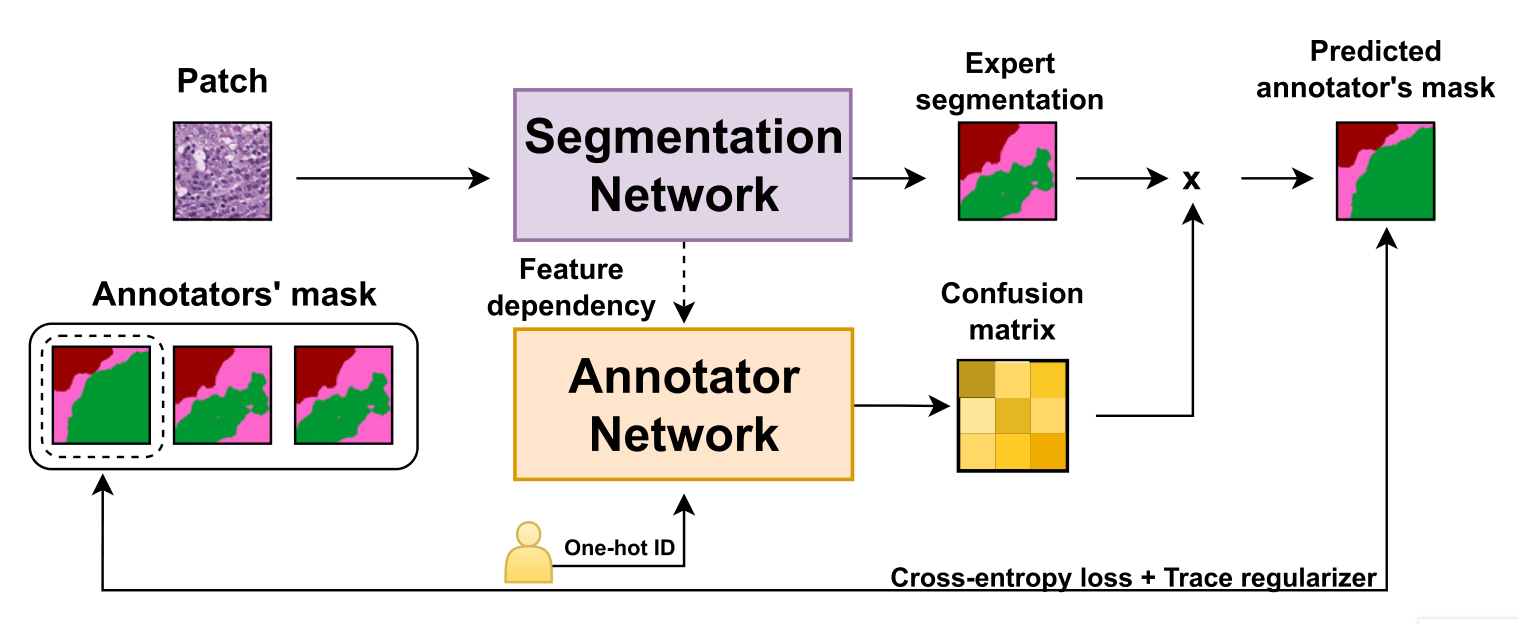
\includegraphics[width=0.7\textwidth]{Cap1/Figures/lopez_2024_proposed_framework.png}
  \caption{Proposed framework for the approach in \cite{LopezEtAl2024}.}
  \label{fig:lopez_2024_proposed_framework}
\end{figure}

Despite the decent performance of the approach, solving the problem
of multiple labelers with two networks can be overwhelming for the
optimization process, requiring large amounts of annotated data to
properly codify the annotators spatial reliabilities, which could be
managed by a single model with an appropriate loss function.
\subsubsection{Bayesian models}\label{subsec:bayesian_models}

Bayesian approaches are a good choice for handling label noise
and uncertainty in the labelers. In \cite{GilEtAlvarez2023CCGPMA} the
authors propose a novel approach from Gaussian Processes to model the
relationship between the annotators' reliability and the input data,
while also preserving the interdependencies among the annotators.
This is achieved by introducing \gls{CCGPMA}, a framework based on
the well known \gls{CGP}.
\gls{CGP} on itself cannot consider inter-annotator dependencies,
thus, the authors introduce the \gls{CCGP} to model correlations
between the GP latent functions, which are supposed to be generated
from a \gls{SLFM}:

\begin{equation}
  f_j(\mathbf{x}_n) = \sum_{q=1}^{Q} w_{j,q} \mu_q(\mathbf{x}_n),
\end{equation}

where $f_j : \mathcal{X} \to \mathbb{R}$ is a \gls{LF}, $\mu_q(\cdot) \sim
\mathcal{GP}(0, k_q(\cdot, \cdot))$ with $k_q : \mathcal{X} \times
\mathcal{X} \to \mathbb{R}$ being a kernel function, and $w_{j,q} \in
\mathbb{R}$ is a combination coefficient ($Q \in \mathbb{N}$). This leads
to a joint distribution of the form:

\begin{equation}
  p(\mathbf{y}, \hat{\mathbf{f}}, u | \mathbf{X}) = p(\mathbf{y} |
  \boldsymbol{\theta}) \prod_{j=1}^{J} p(\mathbf{f}_j | \mathbf{u})
  p(\mathbf{u}),
\end{equation}

where $\mathbf{y}$ is the vector of noisy labels, $\hat{\mathbf{f}}$
is the vector of latent functions, $u$ represents the inducing points,
and $\mathbf{X}$ is the input data.

Combined with inducing-variables based methods for sparse GP
approximations, and maximizing an \gls{ELBO} for the estimation of the
variational parameters, the authors reach a model whose variational
expectations are not analytically tractable, and hence, the authors
derive a Gaussian-Hermite quadrature approach.

Finally, the authors extend this approach for being applied to
classification an regression, reaching the only known approach to
involve chained gaussian processes in multiple annotators
classification and regression tasks while preserving the
interdependencies among the annotators, and also outperforming
GPC-MV\footnote{A GPC using the MV of the labels as the ground truth.},
MA-LFC-C\footnote{A LRC with constant parameters across the input space.},
MA-DGRL\footnote{A multi-labeler approach that considers as latent
variables the annotator performance.},
MA-GPC\footnote{A multi-labeler GPC, which is an extension of MA-LFC.},
MA-GPCV\footnote{An extension of MA-GPC that includes variational
inference and priors over the labelers' parameters.},
MA-DL\footnote{A Crowd Layer for DL, where the annotators' parameters
are constant across the input space.},
KAAR\footnote{A kernel-based approach that employs a convex
combination of classifiers and codes labelers dependencies.}.

\gls{CCGPMA} on itself proposes a good approach for handling label
noise and uncertainty in the labelers for regression and
classification tasks, while also preserving the interdependencies
among the annotators, however, it does not face the image segmentation
problem, which is the main focus of this works, however, it does not
face the image segmentation problem, which is the main focus of this
work. Besides, handling so many latent functions during the
optimization process is computationally expensive, making it on itself
infeasible for large and high resolution datasets.

\subsection{Facing noisy annotations and low-quality data}

The problem of low-quality data and noisy annotations has been
tackled with various strategies. One such approach is the use of deep
learning models that incorporate loss functions designed to mitigate
the effects of unreliable labels. Traditional methods such as
Majority Voting (MV) or Expectation-Maximization (EM) have been
widely used for aggregating multiple annotators' inputs. However,
they assume a homogeneous reliability of annotators, which may not
hold in real-world scenarios.

\subsubsection{Loss functions in deep learning models}

Loss functions are fundamental components in deep learning models
that quantify how well a model's predictions match the ground truth.
They serve as the objective function that guides the learning process
by measuring the discrepancy between predicted and actual values. In
classification tasks, the most common loss functions are
Cross-Entropy (CE) and Mean Absolute Error (MAE)
\cite{ZhangEtAl2018}. CE is particularly
effective for classification as it heavily penalizes confident but
wrong predictions, though it can be sensitive to noisy labels. MAE,
on the other hand, is more robust to outliers and assigns equal
weights to all mistakes, but typically requires more training
iterations. For image segmentation tasks, specialized loss functions
have been developed to handle the unique challenges of pixel-wise
classification. The Dice loss, which measures the overlap between
predicted and ground truth regions, is widely used in medical image
segmentation \cite{ZhaoEtAl2020}. More recently, the Generalized
Cross Entropy (GCE) loss has emerged as a robust alternative that
combines the benefits of both CE and MAE, allowing for better
handling of noisy labels through a tunable parameter that controls
sensitivity to outliers. However, to the best of our knowledge, none
of the current loss functions approaches have focused on the multiple
labelers scenario, neither on the per labeler spatial reliability
estimation.

\subsubsection{Generalized Cross-Entropy for multiple annotators classification}

A more recent approach was proposed by~\cite{TrianaEtAl2023},
introducing a \gls{GCECDL} framework. This method addresses the limitations of
traditional label aggregation techniques by modeling each annotator's
reliability as a function of the input data. The approach effectively
mitigates the impact of noisy labels by using a noise-robust loss
function, balancing Mean Absolute Error (MAE) and Categorical
Cross-Entropy (CE). Unlike prior approaches, \gls{GCECDL} accounts for the
dependencies among annotators while encoding their non-stationary
behavior across different data samples. Their experiments on
multiple datasets demonstrated superior predictive performance
compared to state-of-the-art methods, particularly in cases where
annotations were highly inconsistent.

The strategy of the authors effectively unlocks the potential of
\gls{ML} models to handle low-quality data and noisy annotations, but
it is bounded to classifications tasks only, not being by itself applicable to
segmentation tasks. The TGCE equation for handling multiple
annotators is defined as:

\begin{equation}
  \text{TGCE}(\mathbf{y}, f(\mathbf{x}); \tilde{\lambda}_x,
  \tilde{C}) = \tilde{\lambda}_x \frac{1-(\mathbf{1}^\top(\mathbf{y}
  \odot f(\mathbf{x})))^q}{q} + (1-\tilde{\lambda}_x)\frac{1-(\tilde{C})^q}{q},
\end{equation}

where $\tilde{\lambda}_x$ represents the annotator reliability,
$\tilde{C}$ is a constant, $q$ is a parameter that controls the
balance between MAE and CE behavior, $\mathbf{y}$ is the annotation
vector, and $f(\mathbf{x})$ is the model prediction. This approach is
more deeply discussed in chapter \ref{ch:seg_tgce}.

\begin{table}[htbp]
  \centering
  \caption{Summary of state-of-the-art approaches for handling
  multiple annotators in medical image segmentation}
  \label{tab:state_of_art_summary}
  \begin{tabular}{p{0.2\textwidth}p{0.3\textwidth}p{0.3\textwidth}p{0.15\textwidth}}
    \toprule
    \textbf{Approach} & \textbf{Key Characteristics} &
    \textbf{Advantages} & \textbf{Limitations} \\
    \midrule
    Majority Voting (MV) & Simple aggregation of multiple annotators' labels &
    - Simple to implement
    - No complex algorithms required
    - Proven effective in many cases &
    - Assumes equal expertise
    - Sensitive to correlated errors
    - May introduce bias in expert tasks \\
    \midrule
    STAPLE & Probabilistic framework estimating true segmentation and
    rater reliability &
    - Handles binary and multiclass segmentation
    - Estimates rater sensitivity/specificity
    - Robust to correlated errors &
    - Computationally expensive
    - Sensitive to low-quality annotations
    - Tends to over-smooth results
    - Limited interpretability \\
    \midrule
    U-Net based approaches & Deep learning architecture with
    encoder-decoder structure &
    - Captures both global and local information
    - Effective for complex structures
    - Works well with limited data &
    - Requires large amounts of training data
    - Complex optimization process
    - May need specialized loss functions \\
    \midrule
    Bayesian Models (CCGPMA) & Gaussian Processes modeling annotator
    reliability &
    - Preserves annotator interdependencies
    - Handles label noise effectively
    - Works for classification and regression &
    - Computationally expensive
    - Not directly applicable to segmentation
    - Complex optimization process \\
    \midrule
    Generalized Cross-Entropy (GCE) & Loss function balancing MAE and CE &
    - Robust to noisy labels
    - Accounts for non-stationary behavior
    - Handles annotator dependencies &
    - Limited to classification tasks
    - Requires parameter tuning
    - May need adaptation for segmentation \\
    \bottomrule
  \end{tabular}
\end{table}
